% Options for packages loaded elsewhere
\PassOptionsToPackage{unicode}{hyperref}
\PassOptionsToPackage{hyphens}{url}
%
\documentclass[
]{book}
\usepackage{amsmath,amssymb}
\usepackage{lmodern}
\usepackage{iftex}
\ifPDFTeX
  \usepackage[T1]{fontenc}
  \usepackage[utf8]{inputenc}
  \usepackage{textcomp} % provide euro and other symbols
\else % if luatex or xetex
  \usepackage{unicode-math}
  \defaultfontfeatures{Scale=MatchLowercase}
  \defaultfontfeatures[\rmfamily]{Ligatures=TeX,Scale=1}
\fi
% Use upquote if available, for straight quotes in verbatim environments
\IfFileExists{upquote.sty}{\usepackage{upquote}}{}
\IfFileExists{microtype.sty}{% use microtype if available
  \usepackage[]{microtype}
  \UseMicrotypeSet[protrusion]{basicmath} % disable protrusion for tt fonts
}{}
\makeatletter
\@ifundefined{KOMAClassName}{% if non-KOMA class
  \IfFileExists{parskip.sty}{%
    \usepackage{parskip}
  }{% else
    \setlength{\parindent}{0pt}
    \setlength{\parskip}{6pt plus 2pt minus 1pt}}
}{% if KOMA class
  \KOMAoptions{parskip=half}}
\makeatother
\usepackage{xcolor}
\IfFileExists{xurl.sty}{\usepackage{xurl}}{} % add URL line breaks if available
\IfFileExists{bookmark.sty}{\usepackage{bookmark}}{\usepackage{hyperref}}
\hypersetup{
  pdftitle={A Little Book of R for Bioinformatics 2.0},
  pdfauthor={Avirl Coghlan, with contributions by Nathan L. Brouwer},
  hidelinks,
  pdfcreator={LaTeX via pandoc}}
\urlstyle{same} % disable monospaced font for URLs
\usepackage[margin=1in]{geometry}
\usepackage{listings}
\newcommand{\passthrough}[1]{#1}
\lstset{defaultdialect=[5.3]Lua}
\lstset{defaultdialect=[x86masm]Assembler}
\usepackage{longtable,booktabs,array}
\usepackage{calc} % for calculating minipage widths
% Correct order of tables after \paragraph or \subparagraph
\usepackage{etoolbox}
\makeatletter
\patchcmd\longtable{\par}{\if@noskipsec\mbox{}\fi\par}{}{}
\makeatother
% Allow footnotes in longtable head/foot
\IfFileExists{footnotehyper.sty}{\usepackage{footnotehyper}}{\usepackage{footnote}}
\makesavenoteenv{longtable}
\usepackage{graphicx}
\makeatletter
\def\maxwidth{\ifdim\Gin@nat@width>\linewidth\linewidth\else\Gin@nat@width\fi}
\def\maxheight{\ifdim\Gin@nat@height>\textheight\textheight\else\Gin@nat@height\fi}
\makeatother
% Scale images if necessary, so that they will not overflow the page
% margins by default, and it is still possible to overwrite the defaults
% using explicit options in \includegraphics[width, height, ...]{}
\setkeys{Gin}{width=\maxwidth,height=\maxheight,keepaspectratio}
% Set default figure placement to htbp
\makeatletter
\def\fps@figure{htbp}
\makeatother
\setlength{\emergencystretch}{3em} % prevent overfull lines
\providecommand{\tightlist}{%
  \setlength{\itemsep}{0pt}\setlength{\parskip}{0pt}}
\setcounter{secnumdepth}{5}
\usepackage{booktabs}
\lstset{
  breaklines=true
}
\ifLuaTeX
  \usepackage{selnolig}  % disable illegal ligatures
\fi
\usepackage[]{natbib}
\bibliographystyle{apalike}

\title{A Little Book of R for Bioinformatics 2.0}
\author{Avirl Coghlan, with contributions by Nathan L. Brouwer}
\date{2021-08-15}

\begin{document}
\maketitle

{
\setcounter{tocdepth}{1}
\tableofcontents
}
\hypertarget{preface-to-version-2.0}{%
\chapter*{Preface to version 2.0}\label{preface-to-version-2.0}}
\addcontentsline{toc}{chapter}{Preface to version 2.0}

Welcome to \emph{A Little Book of R for Bioinformatics 2.0}!.

This book is based on the original \href{https://a-little-book-of-r-for-bioinformatics.readthedocs.io/en/latest/}{\emph{A Little Book of R for Bioinformatics}} by Dr.~Avril Coghlan (Hereafter ``ALBRB 1.0''). Dr.~Coghlan's book was one of the first and most thorough introductions to using \emph{R} for bioinformatics and computational biology, and was generously published under the Creative Commons 3.0 Attribution License \href{https://creativecommons.org/licenses/by/3.0/}{(CC BY 3.0)}. In addition to describing how to do bioinformatics in R, Coghlan provided numerous functions to facilitate important tasks, practice questions, and references to further reading.

\href{https://a-little-book-of-r-for-bioinformatics.readthedocs.io/en/latest/}{ALBRB 1.0} was extremely useful to me when I was learning bioinformatics and computational biology. In this version of the book, which I'll refer to as \textbf{ALBRB 2.0}, I have adapted Dr.~Coghlan's original book to suit my own teaching needs, updated it with current packages now available in R, added background materials from other open-access sources, and added in my original materials.

Below I've outlined the general types of changes I've made to the original book. I have tried to link back to the original content that these updates are derived from and note how changes were made. Any errors or inconsistencies should be ascribed to me, not Dr.~Coghlan. If you have any feedback, please email me at \href{mailto:brouwern@gmail.com}{\nolinkurl{brouwern@gmail.com}}

\textasciitilde Nathan Brouwer, June 2021

\textbf{Changes implemented in ALBRB 2.0 by Nathan Brouwer}

\begin{enumerate}
\def\labelenumi{\arabic{enumi}.}
\tightlist
\item
  Converted the entire book to RMarkdown and published it via \passthrough{\lstinline!bookdown!}.
\item
  Added instructions for using RStudio and RStudio Cloud.
\item
  Updated instructions to reflect any changes in software, including changes to how the bioinformatics repository \passthrough{\lstinline!Bioconductor!} now works.
\item
  Split up chapters into smaller units.
\item
  Reorganized the order of some material.
\item
  Added biological background information by integrating information from the Open Access textbook \href{https://bio.libretexts.org/Bookshelves/Introductory_and_General_Biology/Book\%3A_General_Biology_(OpenStax)}{LibreText General Biology}
\item
  Added links to the books I am developing, \emph{Get R Done!} and \emph{Computational Biology for All}.
\item
  Moved functions written by Coghlan and datasets to my teaching package \href{https://github.com/brouwern/compbio4all}{compbio4all}.
\item
  Functions names changed from camelCase to snake\_case
\item
  Functions re-written so as not to use Bioconductor to reduce/eliminate dependency of \passthrough{\lstinline!compbio4all!} on \passthrough{\lstinline!Bioconductor!}.
\item
  Changed some plotting to ggplot2 or ggpubr.
\item
  Added additional subheadings
\item
  Added vocab and function lists to the beginning of many chapters
\item
  At times replaced non-biological examples with biological ones.
\item
  Change from British to American English (Sorry! Couldn't help myself - the spellchecker made me do it!)
\item
  Provided additional links to external resources.
\item
  Added use of \passthrough{\lstinline!rentrez!} for querying NCBI databases
\end{enumerate}

\hypertarget{downloadR}{%
\chapter{Downloading R}\label{downloadR}}

\textbf{By}: Avril Coghlan

\textbf{Adapted, edited and expanded}: Nathan Brouwer (\href{mailto:brouwern@gmail.com}{\nolinkurl{brouwern@gmail.com}}) under the Creative Commons 3.0 Attribution License \href{https://creativecommons.org/licenses/by/3.0/}{(CC BY 3.0)}.

\hypertarget{preface}{%
\section{Preface}\label{preface}}

The following introduction to \emph{R} is based on the first part of \href{https://a-little-book-of-r-for-bioinformatics.readthedocs.io/en/latest/src/installr.html}{``How to install \emph{R} and a Brief Introduction to R''} by Avril Coghlan, which was released under the Creative Commons 3.0 Attribution License \href{https://creativecommons.org/licenses/by/3.0/}{(CC BY 3.0)}. For additional information see the Appendices and \href{https://brouwern.github.io/BOOK_R_Ecological_Data_Science/getting-r-onto-your-computer.html}{``Getting \emph{R} onto your computer''}.

\hypertarget{introduction-to-r}{%
\section{Introduction to R}\label{introduction-to-r}}

\emph{R} (www.r-project.org) is a commonly used free statistics software. \emph{R} allows you to carry out statistical analyses in an interactive mode, as well as allowing programming.

\hypertarget{installing-r}{%
\section{Installing R}\label{installing-r}}

To use R, you first need to install the \emph{R} program on your computer.

\hypertarget{installing-r-on-a-windows-pc}{%
\subsection{\texorpdfstring{Installing \emph{R} on a Windows PC}{Installing R on a Windows PC}}\label{installing-r-on-a-windows-pc}}

These instructions will focus on installing \emph{R} on a Windows PC. However, I will also briefly mention how to install \emph{R} on a Macintosh or Linux computer (see below).

\textbf{These steps have not been checked as of 8/13/2019 so there may be small variations in what the prompts are. Installing R, however, is basically that same as any other program. Clicking ``Yes'' etc on everything should work.}

\begin{quote}
\textbf{PROTIP:} Even if you have used \emph{R} before its good to regularly update it to avoid conflicts with recently produced software.
\end{quote}

Minor updates of \emph{R} are made very regularly (approximately every 6 months), as \emph{R} is actively being improved all the time. It is worthwhile installing new versions of \emph{R} a couple times a year, to make sure that you have a recent version of \emph{R} (to ensure compatibility with all the latest versions of the \emph{R} packages that you have downloaded).

To install \emph{R} on your \textbf{Windows} computer, follow these steps:

\begin{enumerate}
\def\labelenumi{\arabic{enumi}.}
\tightlist
\item
  Go to \url{https://cran.r-project.org/}
\item
  Under ``Download and Install R'', click on the ``Windows'' link.
\item
  Under ``Subdirectories'', click on the \textbf{``base''} link.
\item
  On the next page, you should see a link saying something like ``Download \emph{R} 4.1.0 for Windows'' (or \emph{R} X.X.X, where X.X.X gives the version of the program). Click on this link.
\item
  You may be asked if you want to save or run a file ``R-x.x.x-win32.exe''. Choose ``Save'' and save the file. Then double-click on the icon for the file to run it.
\item
  You will be asked what language to install it in.
\item
  The \emph{R} Setup Wizard will appear in a window. Click ``Next'' at the bottom of the \emph{R} Setup wizard window.
\item
  The next page says ``Information'' at the top. Click ``Next'' again.
\item
  The next page says ``Select Destination Location'' at the top. By default, it will suggest to install \emph{R} on the C drive in the ``Program Files'' directory on your computer.
\item
  Click ``Next'' at the bottom of the \emph{R} Setup wizard window.
\item
  The next page says ``Select components'' at the top. Click ``Next'' again.
\item
  The next page says ``Startup options'' at the top. Click ``Next'' again.
\item
  The next page says ``Select start menu folder'' at the top. Click ``Next'' again.
\item
  The next page says ``Select additional tasks'' at the top. Click ``Next'' again.
\item
  \emph{R} should now be installing. This will take about a minute. When \emph{R} has finished, you will see ``Completing the \emph{R} for Windows Setup Wizard'' appear. Click ``Finish''.
\item
  To start R, you can do one of the following steps:
\item
  Check if there is an ``R'' icon on the desktop of the computer that you are using. If so, double-click on the ``R'' icon to start R. If you cannot find an ``R'' icon, try the next step instead.
\item
  Click on the ``Start'' button at the bottom left of your computer screen, and then choose ``All programs'', and start \emph{R} by selecting ``R'' (or \emph{R} X.X.X, where X.X.X gives the version of R) from the menu of programs.
\item
  The \emph{R} console (a rectangle) should pop up:
\end{enumerate}

\hypertarget{how-to-install-r-on-non-windows-computers-eg.-macintosh-or-linux-computers}{%
\subsection{\texorpdfstring{How to install \emph{R} on non-Windows computers (eg. Macintosh or Linux computers)}{How to install R on non-Windows computers (eg. Macintosh or Linux computers)}}\label{how-to-install-r-on-non-windows-computers-eg.-macintosh-or-linux-computers}}

\textbf{These steps have not been checked as of 8/13/2019 so there may be small variations in what the prompts are. Installing R, however, is basically that same as any other program. Clicking ``Yes'' etc on everything should work.}

The instructions above are for installing \emph{R} on a Windows PC. If you want to install \emph{R} on a computer that has a non-Windows operating system (for example, a Macintosh or computer running Linux, you should download the appropriate \emph{R} installer for that operating system at \url{https://cran.r-project.org/} and follow the \emph{R} installation instructions for the appropriate operating system at \url{https://cran.r-project.org/doc/FAQ/R-FAQ.html\#How-can-R-be-installed_003f} .

\hypertarget{starting-r}{%
\section{\texorpdfstring{Starting \emph{R}}{Starting R}}\label{starting-r}}

To start R, Check if there is an \emph{R} icon on the desktop of the computer that you are using. If so, double-click on the \emph{R} icon to start \emph{R}. If you cannot find an \emph{R} icon, try the next step instead.

You can also start \emph{R} from the Start menu in Windows. Click on the ``Start'' button at the bottom left of your computer screen, and then choose ``All programs'', and start \emph{R} by selecting ``R'' (or \emph{R} X.X.X, where X.X.X gives the version of R, e.g.. \emph{R} 2.10.0) from the menu of programs.

Say ``Hi'' to \emph{R} and take a quick look at how it looks. Now say ``Goodbye'', because we will never actually do any work in this version of \emph{R}; instead, we'll use the \textbf{RStudio IDE (integrated development environment)}.

\hypertarget{installing-the-rstudio-ide-installrstudio}{%
\chapter{Installing the RStudio IDE \{\$installRStudio\}}\label{installing-the-rstudio-ide-installrstudio}}

\textbf{By:} Nathan Brouwer

The name ``R'' refers both to the programming language and the program that runs that language. When you download \emph{it}R* there is also a basic \textbf{GUI} (graphical user interface) that you can access via the \emph{R} icon.

Other GUIs are available, and the most popular currently is \textbf{RStudio.} RStudio a for-profit company that is a main driver of development of R. Much of what they produce has free basic versions or is entirely free. They produce software (RStudio), cloud-based applications (\textbf{RStudio Cloud}), and web server infrastructure for business applications of R.

A brief overview of installing RStudio can be found here \href{https://brouwern.github.io/BOOK_R_Ecological_Data_Science/getting-rstudio-on-to-your-computer.html}{``Getting RStudio on to your computer''}

\hypertarget{getting-to-know-rstudio}{%
\section{Getting to know RStudio}\label{getting-to-know-rstudio}}

For a brief overview of RStudio see \href{https://brouwern.github.io/BOOK_R_Ecological_Data_Science/getting-started-with-rstudio.html}{``Getting started with RStudio''}

A good overview of what the different parts of RStudio can be seen in the image in this tweet: \url{https://twitter.com/RLadiesNCL/status/1138812826917724160?s=20}

\hypertarget{rstudio-versus-rstudio-cloud}{%
\section{RStudio versus RStudio Cloud}\label{rstudio-versus-rstudio-cloud}}

RStudio and RStudio cloud work almost identically, so anything you read about RStudio will apply to RStudio Cloud. RStudio is easy to download an use, but RStudio Cloud eliminates even the minor hiccups that occur. Free accounts with RStudio Cloud allow up to 15 hours per month, which is enough for you to get a taste for using R.

\hypertarget{installing-packages}{%
\chapter{\texorpdfstring{Installing \emph{R} packages}{Installing R packages}}\label{installing-packages}}

\textbf{By}: Avril Coghlan.

\textbf{Adapted, edited and expanded}: Nathan Brouwer under the Creative Commons 3.0 Attribution License \href{https://creativecommons.org/licenses/by/3.0/}{(CC BY 3.0)}.

\emph{R} is a programming language, and \textbf{packages} (aka \textbf{libraries}) are bundles of software built using \emph{R}. Most sessions using \emph{R} involve using additional \emph{R} packages. This is especially true for bioinformatics and computational biology.

\begin{quote}
\textbf{NOTE}: If you are working in an RStudio Cloud environment organized by someone else (e.g.~a course instructor), they likely are taking care of many of the package management issues. The following information is still useful to be familiar with.
\end{quote}

\hypertarget{downloading-packages-with-the-rstudio-ide}{%
\section{Downloading packages with the RStudio IDE}\label{downloading-packages-with-the-rstudio-ide}}

There is a point-and-click interface for installing \emph{R} packages in RStudio. There is a brief introduction to downloading packages on this site: \url{http://web.cs.ucla.edu/~gulzar/rstudio/}

I've summarized it here:

\begin{enumerate}
\def\labelenumi{\arabic{enumi}.}
\tightlist
\item
  ``Click on the''Packages'' tab in the bottom-right section and then click on ``Install''. The following dialog box will appear.
\item
  In the ``Install Packages'' dialog, write the package name you want to install under the Packages field and then click install. This will install the package you searched for or give you a list of matching package based on your package text.
\end{enumerate}

\hypertarget{downloading-packages-with-the-function-install.packages}{%
\section{\texorpdfstring{Downloading packages with the function \texttt{install.packages()}}{Downloading packages with the function install.packages()}}\label{downloading-packages-with-the-function-install.packages}}

The easiest way to install a package if you know its name is to use the \emph{R} function \passthrough{\lstinline!install.packages(!})`. Note that it might be better to call this ``download.packages'' since after you install it, you also have to load it!

Frequently I will include \passthrough{\lstinline!install.packages(...)!} at the beginning of a chapter the first time we use a package to make sure the package is downloaded. Note, however, that if you already have downloaded the package, running \passthrough{\lstinline!install.packages(...)!} will download a new copy. While packages do get updated from time to time, but its best to re-run \passthrough{\lstinline!install.packages(...)!} only occassionaly.

We'll download a package used for plotting called \passthrough{\lstinline!ggplot2!}, which stands for ``Grammar of Graphics.'' \passthrough{\lstinline!ggplot2!} was developed by Dr.~\href{http://hadley.nz/}{Hadley Wickham}, who is now the Chief Scientists for RStudio.

To download \passthrough{\lstinline!ggplot2!}, run the following command:

\begin{lstlisting}[language=R]
install.packages("ggplot2") # note the " "
\end{lstlisting}

Often when you download a package you'll see a fair bit of angry-looking red text, and sometime other things will pop up. Usually there's nothing of interest here, but sometimes you need to read things carefully over it for hints about why something didn't work.

\hypertarget{using-packages-after-they-are-downloaded}{%
\section{Using packages after they are downloaded}\label{using-packages-after-they-are-downloaded}}

To actually make the functions in package accessible you need to use the \passthrough{\lstinline!library()!} command. Note that this is \emph{not} in quotes.

\begin{lstlisting}[language=R]
library(ggplot2) # note: NO " "
\end{lstlisting}

\hypertarget{installing-bioconductor}{%
\chapter{Installing Bioconductor}\label{installing-bioconductor}}

\textbf{By}: Avril Coghlan.

\textbf{Adapted, edited and expanded}: Nathan Brouwer under the Creative Commons 3.0 Attribution License \href{https://creativecommons.org/licenses/by/3.0/}{(CC BY 3.0)}, including details on install Bioconductor and common prompts and error messages that appear during installation.

\hypertarget{bioconductor}{%
\section{Bioconductor}\label{bioconductor}}

\emph{R} \textbf{packages} (aka ``libraries'') can live in many places. Most are accessed via \textbf{CRAN}, the \textbf{Comprehensive R Archive Network}. The bioinformatics and computational biology community also has its own package hosting system called \href{www.bioconductor.org}{Bioconductor}. \emph{R} has played an important part in the development and application of bioinformatics techniques in the 21th century. Bioconductor 1.0 was released in 2002 with 15 packages. As of winter 2021, there are almost 2000 packages in the current release!

\begin{quote}
\textbf{NOTE}: If you are working in an RStudio Cloud environment organized by someone else (eg a course instructor), they likely are taking care of most of package management issues, inlcuding setting up Bioconductor. The following information is still useful to be familiar with.
\end{quote}

To interface with Bioconductor you need the \href{https://cran.r-project.org/web/packages/BiocManager/vignettes/BiocManager.html}{BiocManager} package. The Bioconductor people have put \href{https://cran.r-project.org/web/packages/BiocManager/vignettes/BiocManager.html}{BiocManager} on CRAN to allow you to set up interactions with Bioconductor. See the \href{https://cran.r-project.org/web/packages/BiocManager/vignettes/BiocManager.html}{BiocManager documentation} for more information (\url{https://cran.r-project.org/web/packages/BiocManager/vignettes/BiocManager.html}).

Note that if you have an old version of R you will need to update it to interact with Bioconductor.

\hypertarget{installing-biocmanager}{%
\section{Installing BiocManager}\label{installing-biocmanager}}

BiocManager can be installed using the \passthrough{\lstinline!install.packages()!} packages command.

\begin{lstlisting}[language=R]
install.packages("BiocManager") # Remember the "  "; don't worry about the red text
\end{lstlisting}

Once downloaded, BioManager needs to be explicitly loaded into your active R session using \passthrough{\lstinline!library()!}

\begin{lstlisting}[language=R]
library(BiocManager) # no quotes; again, ignore the red text
\end{lstlisting}

Individual Bioconductor packages can then be downloaded using the \passthrough{\lstinline!install()!} command. An essential packages is \passthrough{\lstinline!Biostrings!}. To do this ,

\begin{lstlisting}[language=R]
BiocManager::install("Biostrings")
\end{lstlisting}

\hypertarget{the-ins-and-outs-of-package-installation}{%
\section{The ins and outs of package installation}\label{the-ins-and-outs-of-package-installation}}

\textbf{IMPORANT} Bioconductor has many \textbf{dependencies} - other packages which is relies on. When you install Bioconductor packages you may need to update these packages. If something seems to not be working during this process, restart R and begin the Bioconductor installation process until things seem to work.

Below I discuss the series of prompts I had to deal with while re-installing Biostrings while editing this chapter.

\hypertarget{updating-other-packages-when-downloading-a-package}{%
\subsection{Updating other packages when downloading a package}\label{updating-other-packages-when-downloading-a-package}}

When I re-installed \passthrough{\lstinline!Biostrings!} while writing this I was given a HUGE blog of red test that contained something like what's shown below (this only aout 1/3 of the actual output!):

\begin{lstlisting}[language=R]
'getOption("repos")' replaces Bioconductor standard repositories, 
see '?repositories' for details

replacement repositories:
    CRAN: https://cran.rstudio.com/

Bioconductor version 3.11 (BiocManager 1.30.16), R 4.0.5 (2021-03-31)
Old packages: 'ade4', 'ape', 'aster', 'bayestestR', 
  'bio3d', 'bitops', 'blogdown',
  'bookdown', 'brio', 'broom', 'broom.mixed', 
  'broomExtra', 'bslib', 'cachem', 'callr',
  'car', 'circlize', 'class', 'cli', 'cluster', 
  'colorspace', 'corrplot', 'cpp11', 'curl',
  'devtools', 'DHARMa', 'doBy', 'dplyr', 'DT', 
  'e1071', 'ellipsis', 'emmeans', 'emojifont',
  'extRemes', 'fansi', 'flextable', 'forecast', 
  'formatR', 'gap', 'gargle', 'gert', 'GGally'
\end{lstlisting}

Hidden at the bottom was a prompt:
\passthrough{\lstinline!"Update all/some/none? [a/s/n]:"!}

Its a little vague, but what it wants me to do is type in \passthrough{\lstinline!a!}, \passthrough{\lstinline!s!} or \passthrough{\lstinline!n!} and press enter to tell it what to do. I almost always chose \passthrough{\lstinline!a!}, though this may take a while to update everything.

\hypertarget{packages-from-source}{%
\subsection{Packages ``from source''}\label{packages-from-source}}

You are likely to get lots of random-looking feedback from R when doing Bioconductor-related installations. Look carefully for any prompts as the very last line. While updating \passthrough{\lstinline!Biostrings!} I was told: ``\emph{There are binary versions available but the source versions are later:}'' and given a table of packages. I was then asked ``\emph{Do you want to install from sources the packages which need compilation? (Yes/no/cancel)}''

I almost always chose ``no''.

\hypertarget{more-on-angry-red-text}{%
\subsection{More on angry red text}\label{more-on-angry-red-text}}

After the prompt about packages from source, R proceeded to download a lot of updates to packages, which took a few minutes. Lots of red text scrolled by, but this is normal.

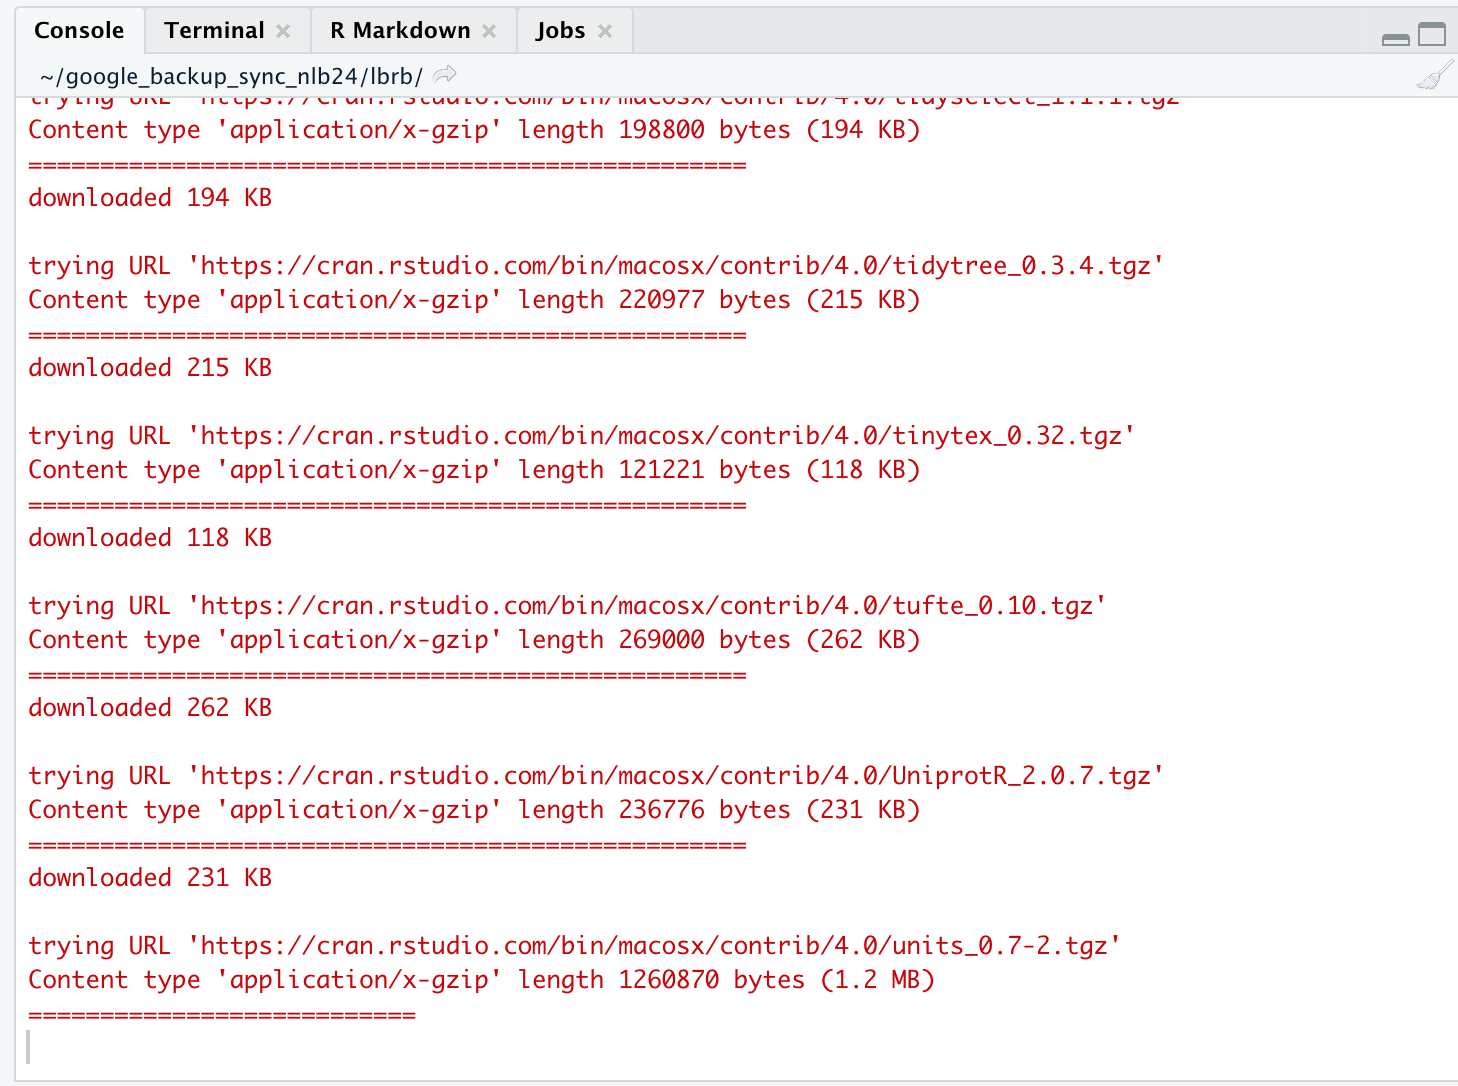
\includegraphics[width=0.4\linewidth]{images/angry_red_text_download_biostrings}

\hypertarget{actually-loading-a-package}{%
\section{Actually loading a package}\label{actually-loading-a-package}}

Again, to actually load the \passthrough{\lstinline!Biostrings!} package into your active R sessions requires the \passthrough{\lstinline!libary()!} command:

\begin{lstlisting}[language=R]
library(Biostrings)
\end{lstlisting}

As you might expect, there's more red text scrolling up my screen!

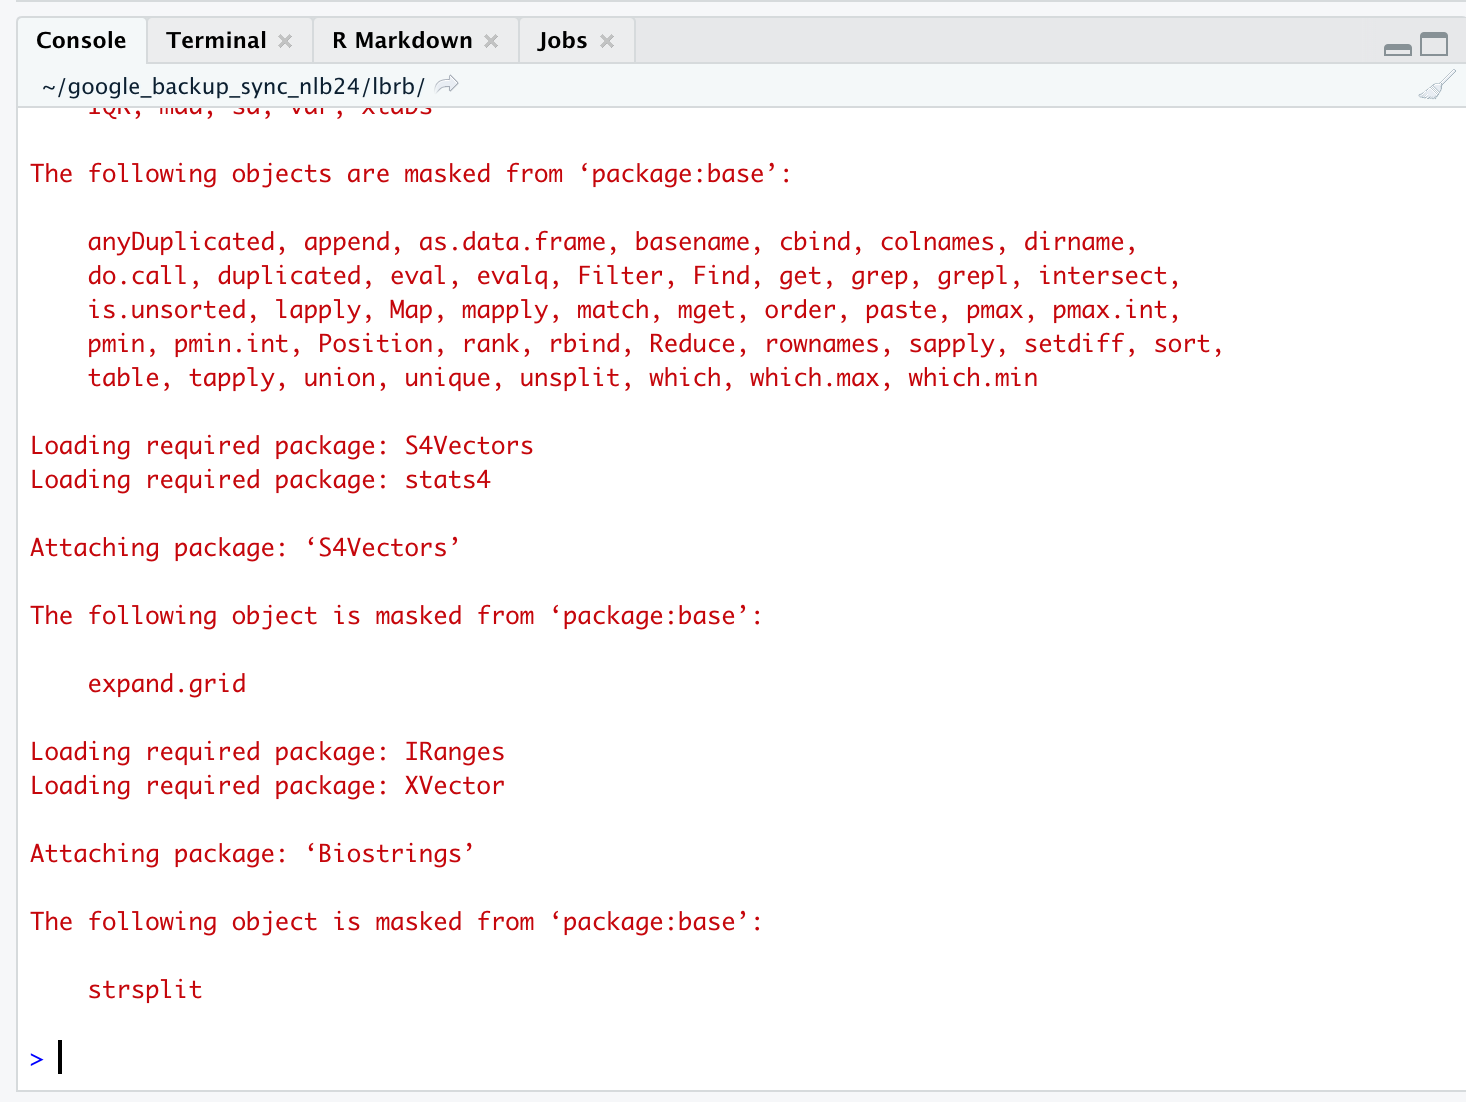
\includegraphics[width=0.4\linewidth]{images/angry_red_text_library_biostrings}

I can tell that is actually worked because at the end of all the red stuff is the R prompt of ``\textgreater{}'' and my cursor.

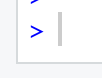
\includegraphics[width=1.42in]{images/R_cursor}

\hypertarget{basic-R}{%
\chapter{A Brief introduction to R}\label{basic-R}}

\textbf{By}: Avril Coghlan.

\textbf{Adapted, edited and expanded}: Nathan Brouwer under the Creative Commons 3.0 Attribution License \href{https://creativecommons.org/licenses/by/3.0/}{(CC BY 3.0)}.

This chapter provides a brief introduction to R. At the end of are links to additional resources for getting started with R.

\hypertarget{vocabulary}{%
\section{Vocabulary}\label{vocabulary}}

\begin{itemize}
\tightlist
\item
  scalar
\item
  vector
\item
  list
\item
  class
\item
  numeric
\item
  character
\item
  assignment
\item
  elements of an object
\item
  indices
\item
  attributes of an object
\item
  argument of a function
\end{itemize}

\hypertarget{r-functions}{%
\section{R functions}\label{r-functions}}

\begin{itemize}
\tightlist
\item
  \textless-
\item
  {[} {]}
\item
  \$
\item
  table()
\item
  function
\item
  c()
\item
  log10()
\item
  help(), ?
\item
  help.search()
\item
  RSiteSearch()
\item
  mean()
\item
  return()
\item
  q()
\end{itemize}

\hypertarget{interacting-with-r}{%
\section{Interacting with R}\label{interacting-with-r}}

You will type \emph{R} commands into the RStudio \textbf{console} in order to carry out analyses in \emph{R}. In the RStudio console you will see the R prompt starting with the symbol ``\textgreater{}''. ``\textgreater{}'' will always be there at the beginning of each new command - don't try to delete it! Moreover, you never need to type it.

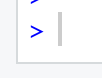
\includegraphics[width=1.42in]{images/R_cursor}

We type the \textbf{commands} needed for a particular task after this prompt. The command is carried out by \emph{R} after you hit the Return key.

Once you have started R, you can start typing commands into the RStudio console, and the results will be calculated immediately, for example:

\begin{lstlisting}[language=R]
2*3
\end{lstlisting}

\begin{lstlisting}
## [1] 6
\end{lstlisting}

Note that prior to the output of ``6'' it shows ``{[}1{]}''.

Now subtraction:

\begin{lstlisting}[language=R]
10-3
\end{lstlisting}

\begin{lstlisting}
## [1] 7
\end{lstlisting}

Again, prior to the output of ``7'' it shows ``{[}1{]}''.

\emph{R} can act like a basic calculator that you type commands in to. You can also use it like a more advanced scientific calculator and create \textbf{variables} that store information. All variables created by R are called \textbf{objects}. In R, we assign values to variables using an arrow-looking function \passthrough{\lstinline!<-!} the \textbf{assignment operator}. For example, we can \textbf{assign} the value 2*3 to the variable x using the command:

\begin{lstlisting}[language=R]
x <- 2*3
\end{lstlisting}

To view the contents of any R object, just type its name, press enter, and the contents of that R object will be displayed:

\begin{lstlisting}[language=R]
x
\end{lstlisting}

\begin{lstlisting}
## [1] 6
\end{lstlisting}

\hypertarget{variables-in-r}{%
\section{Variables in R}\label{variables-in-r}}

There are several different types of objects in R with fancy math names, including \textbf{scalars}, \textbf{vectors}, \textbf{matrices} (singular: \textbf{matrix), }arrays\textbf{, }dataframes\textbf{, }tables\textbf{, and }lists\textbf{. The }scalar** variable x above is one example of an R object. While a scalar variable such as x has just one element, a \textbf{vector} consists of several elements. The elements in a vector are all of the same \textbf{type} (e.g.. numbers or alphabetic characters), while \textbf{lists} may include elements such as characters as well as numeric quantities. Vectors and dataframes are the most common variables you'll use. You'll also encounter matrices often, and lists are ubiquitous in R but beginning users often don't encounter them because they remain behind the scenes.

\hypertarget{vectors}{%
\subsection{Vectors}\label{vectors}}

To create a vector, we can use the \passthrough{\lstinline!c()!} (combine) function. For example, to create a vector called \passthrough{\lstinline!myvector!} that has elements with values 8, 6, 9, 10, and 5, we type:

\begin{lstlisting}[language=R]
myvector <- c(8, 6, 9, 10, 5) # note: commas between each number!
\end{lstlisting}

To see the contents of the variable \passthrough{\lstinline!myvector!}, we can just type its name and press enter:

\begin{lstlisting}[language=R]
myvector
\end{lstlisting}

\begin{lstlisting}
## [1]  8  6  9 10  5
\end{lstlisting}

\hypertarget{vector-indexing}{%
\subsection{Vector indexing}\label{vector-indexing}}

The \passthrough{\lstinline![1]!} is the \textbf{index} of the first \textbf{element} in the vector. We can \textbf{extract} any element of the vector by typing the vector name with the index of that element given in \textbf{square brackets} \passthrough{\lstinline![...]!}.

For example, to get the value of the 4th element in the vector \passthrough{\lstinline!myvector!}, we type:

\begin{lstlisting}[language=R]
myvector[4]
\end{lstlisting}

\begin{lstlisting}
## [1] 10
\end{lstlisting}

\hypertarget{character-vectors}{%
\subsection{Character vectors}\label{character-vectors}}

Vectors can contain letters, such as those designating nucleic acids

\begin{lstlisting}[language=R]
my.seq <- c("A","T","C","G")
\end{lstlisting}

They can also contain multi-letter \textbf{strings}:

\begin{lstlisting}[language=R]
my.oligos <- c("ATCGC","TTTCGC","CCCGCG","GGGCGC")
\end{lstlisting}

\hypertarget{lists}{%
\subsection{Lists}\label{lists}}

\textbf{NOTE}: \emph{below is a discussion of lists in R. This is excellent information, but not necessary if this is your very very first time using R.}

In contrast to a vector, a \textbf{list} can contain elements of different types, for example, both numbers and letters. A list can even include other variables such as a vector. The \passthrough{\lstinline!list()!} function is used to create a list. For example, we could create a list \passthrough{\lstinline!mylist!} by typing:

\begin{lstlisting}[language=R]
mylist <- list(name="Charles Darwin", 
               wife="Emma Darwin", 
               myvector)
\end{lstlisting}

We can then print out the contents of the list \passthrough{\lstinline!mylist!} by typing its name:

\begin{lstlisting}[language=R]
mylist
\end{lstlisting}

\begin{lstlisting}
## $name
## [1] "Charles Darwin"
## 
## $wife
## [1] "Emma Darwin"
## 
## [[3]]
## [1]  8  6  9 10  5
\end{lstlisting}

The \textbf{elements} in a list are numbered, and can be referred to using \textbf{indices}. We can extract an element of a list by typing the list name with the index of the element given in double \textbf{square brackets} (in contrast to a vector, where we only use single square brackets).

We can extract the second element from \passthrough{\lstinline!mylist!} by typing:

\begin{lstlisting}[language=R]
mylist[[2]]  # note the double square brackets [[...]]
\end{lstlisting}

\begin{lstlisting}
## [1] "Emma Darwin"
\end{lstlisting}

As a baby step towards our next task, we can wrap index values as in the \passthrough{\lstinline!c()!} command like this:

\begin{lstlisting}[language=R]
mylist[[c(2)]]  # note the double square brackets [[...]]
\end{lstlisting}

\begin{lstlisting}
## [1] "Emma Darwin"
\end{lstlisting}

The number \passthrough{\lstinline!2!} and \passthrough{\lstinline!c(2)!} mean the same thing.

Now, we can extract the second AND third elements from \passthrough{\lstinline!mylist!}. First, we put the indices 2 and 3 into a vector \passthrough{\lstinline!c(2,3)!}, then wrap that vector in double square brackets: \passthrough{\lstinline![c(2,3)]!}. All together it looks like this.

\begin{lstlisting}[language=R]
mylist[c(2,3)] # note the double brackets
\end{lstlisting}

\begin{lstlisting}
## $wife
## [1] "Emma Darwin"
## 
## [[2]]
## [1]  8  6  9 10  5
\end{lstlisting}

Elements of lists may also be named, resulting in a \textbf{named lists}. The elements may then be referred to by giving the list name, followed by ``\$'', followed by the element name. For example, mylist\$name is the same as mylist{[}{[}1{]}{]} and mylist\$wife is the same as mylist{[}{[}2{]}{]}:

\begin{lstlisting}[language=R]
mylist$wife
\end{lstlisting}

\begin{lstlisting}
## [1] "Emma Darwin"
\end{lstlisting}

We can find out the names of the named elements in a list by using the \passthrough{\lstinline!attributes()!} function, for example:

\begin{lstlisting}[language=R]
attributes(mylist)
\end{lstlisting}

\begin{lstlisting}
## $names
## [1] "name" "wife" ""
\end{lstlisting}

When you use the \passthrough{\lstinline!attributes()!} function to find the named elements of a list variable, the named elements are always listed under a heading ``\$names''. Therefore, we see that the named elements of the list variable \passthrough{\lstinline!mylist!} are called ``name'' and ``wife'', and we can retrieve their values by typing mylist\$name and mylist\$wife, respectively.

\hypertarget{tables}{%
\subsection{Tables}\label{tables}}

Another type of object that you will encounter in R is a \textbf{table}. The \passthrough{\lstinline!table()!} function allows you to total up or tabulate the number of times a value occurs within a vector. Tables are typically used on vectors containing \textbf{character data}, such as letters, words, or names, but can work on numeric data data.

\hypertarget{tables---the-basics}{%
\subsubsection{Tables - The basics}\label{tables---the-basics}}

If we made a vector variable ``nucleotides'' containing the of a DNA molecule, we can use the \passthrough{\lstinline!table()!} function to produce a \textbf{table variable} that contains the number of bases with each possible nucleotides:

\begin{lstlisting}[language=R]
bases <- c("A", "T", "A", "A", "T", "C", "G", "C", "G")
\end{lstlisting}

Now make the table

\begin{lstlisting}[language=R]
table(bases)
\end{lstlisting}

\begin{lstlisting}
## bases
## A C G T 
## 3 2 2 2
\end{lstlisting}

We can store the table variable produced by the function \passthrough{\lstinline!table()!}, and call the stored table ``bases.table'', by typing:

\begin{lstlisting}[language=R]
bases.table <- table(bases)
\end{lstlisting}

Tables also work on vectors containing numbers. First, a vector of numbers.

\begin{lstlisting}[language=R]
numeric.vecter <- c(1,1,1,1,3,4,4,4,4)
\end{lstlisting}

Second, a table, showing how many times each number occurs.

\begin{lstlisting}[language=R]
table(numeric.vecter)
\end{lstlisting}

\begin{lstlisting}
## numeric.vecter
## 1 3 4 
## 4 1 4
\end{lstlisting}

\hypertarget{tables---further-details}{%
\subsubsection{Tables - further details}\label{tables---further-details}}

To access elements in a table variable, you need to use double square brackets, just like accessing elements in a list. For example, to access the fourth element in the table bases.table (the number of Ts in the sequence), we type:

\begin{lstlisting}[language=R]
bases.table[[4]]  # double brackets!
\end{lstlisting}

\begin{lstlisting}
## [1] 2
\end{lstlisting}

Alternatively, you can use the name of the fourth element in the table (``John'') to find the value of that table element:

\begin{lstlisting}[language=R]
bases.table[["T"]]
\end{lstlisting}

\begin{lstlisting}
## [1] 2
\end{lstlisting}

\hypertarget{arguments}{%
\section{Arguments}\label{arguments}}

Functions in R usually require \textbf{arguments}, which are input variables (i.e.. objects) that are \textbf{passed} to them, which they then carry out some operation on. For example, the \passthrough{\lstinline!log10()!} function is passed a number, and it then calculates the log to the base 10 of that number:

\begin{lstlisting}[language=R]
log10(100)
\end{lstlisting}

\begin{lstlisting}
## [1] 2
\end{lstlisting}

There's a more generic function, \passthrough{\lstinline!log()!}, where we pass it not only a number to take the log of, but also the specific \textbf{base} of the logarithm. To take the log base 10 with the \passthrough{\lstinline!log()!} function we do this

\begin{lstlisting}[language=R]
log(100, base = 10)
\end{lstlisting}

\begin{lstlisting}
## [1] 2
\end{lstlisting}

We can also take logs with other bases, such as 2:

\begin{lstlisting}[language=R]
log(100, base = 2)
\end{lstlisting}

\begin{lstlisting}
## [1] 6.643856
\end{lstlisting}

\hypertarget{help-files-with-help-and}{%
\section{\texorpdfstring{Help files with \texttt{help()} and \texttt{?}}{Help files with help() and ?}}\label{help-files-with-help-and}}

In \emph{R}, you can get help about a particular function by using the \passthrough{\lstinline!help()!} function. For example, if you want help about the \passthrough{\lstinline!log10()!} function, you can type:

\begin{lstlisting}[language=R]
help("log10")
\end{lstlisting}

When you use the \passthrough{\lstinline!help()!} function, a box or web page will show up in one of the panes of RStudio with information about the function that you asked for help with. You can also use the \passthrough{\lstinline!?!} next to the function like this

\begin{lstlisting}[language=R]
?log10
\end{lstlisting}

Help files are a mixed bag in R, and it can take some getting used to them. An excellent overview of this is Kieran Healy's \href{https://socviz.co/appendix.html}{``How to read an R help page.''}

\hypertarget{searching-for-functions-with-help.search-and-rsitesearch}{%
\section{\texorpdfstring{Searching for functions with \texttt{help.search()} and \texttt{RSiteSearch()}}{Searching for functions with help.search() and RSiteSearch()}}\label{searching-for-functions-with-help.search-and-rsitesearch}}

If you are not sure of the name of a function, but think you know part of its name, you can search for the function name using the \passthrough{\lstinline!help.search()!} and \passthrough{\lstinline!RSiteSearch()!} functions. The \passthrough{\lstinline!help.search()!} function searches to see if you already have a function installed (from one of the R packages that you have installed) that may be related to some topic you're interested in. \passthrough{\lstinline!RSiteSearch()!} searches \emph{all} R functions (including those in packages that you haven't yet installed) for functions related to the topic you are interested in.

For example, if you want to know if there is a function to calculate the standard deviation (SD) of a set of numbers, you can search for the names of all installed functions containing the word ``deviation'' in their description by typing:

\begin{lstlisting}[language=R]
help.search("deviation")
\end{lstlisting}

Among the functions that were found, is the function \passthrough{\lstinline!sd()!} in the \passthrough{\lstinline!stats!} package (an R package that comes with the base R installation), which is used for calculating the standard deviation.

Now, instead of searching just the packages we've have on our computer let's search all R packages on CRAN. Let's look for things related to DNA. Note that \passthrough{\lstinline!RSiteSearch()!} doesn't provide output within RStudio, but rather opens up your web browser for you to display the results.

\begin{lstlisting}[language=R]
RSiteSearch("DNA")
\end{lstlisting}

The results of the \passthrough{\lstinline!RSiteSearch()!} function will be hits to descriptions of R functions, as well as to R mailing list discussions of those functions.

\hypertarget{more-on-functions}{%
\section{More on functions}\label{more-on-functions}}

We can perform computations with R using objects such as scalars and vectors. For example, to calculate the average of the values in the vector \passthrough{\lstinline!myvector!} (i.e.. the average of 8, 6, 9, 10 and 5), we can use the \passthrough{\lstinline!mean()!} function:

\begin{lstlisting}[language=R]
mean(myvector) # note: no " "
\end{lstlisting}

\begin{lstlisting}
## [1] 7.6
\end{lstlisting}

We have been using built-in R functions such as mean(), length(), print(), plot(), etc.

\hypertarget{writing-your-own-functions}{%
\subsection{Writing your own functions}\label{writing-your-own-functions}}

\textbf{NOTE}: *Writing your own functions is an advanced skills. New users can skip this section.

We can also create our own functions in R to do calculations that you want to carry out very often on different input data sets. For example, we can create a function to calculate the value of 20 plus square of some input number:

\begin{lstlisting}[language=R]
myfunction <- function(x) { return(20 + (x*x)) }
\end{lstlisting}

This function will calculate the square of a number (x), and then add 20 to that value. The \passthrough{\lstinline!return()!} statement returns the calculated value. Once you have typed in this function, the function is then available for use. For example, we can use the function for different input numbers (e.g.. 10, 25):

\begin{lstlisting}[language=R]
myfunction(10)
\end{lstlisting}

\begin{lstlisting}
## [1] 120
\end{lstlisting}

\hypertarget{quiting-r}{%
\section{Quiting R}\label{quiting-r}}

To quit R either close the program, or type:

\begin{lstlisting}[language=R]
q()
\end{lstlisting}

\hypertarget{links-and-further-reading}{%
\section{Links and Further Reading}\label{links-and-further-reading}}

Some links are included here for further reading.

For a more in-depth introduction to R, a good online tutorial is available on the ``Kickstarting R'' website, cran.r-project.org/doc/contrib/Lemon-kickstart.

There is another nice (slightly more in-depth) tutorial to R available on the ``Introduction to R'' website, cran.r-project.org/doc/manuals/R-intro.html.

\href{https://learningstatisticswithr.com/book/introR.html}{Chapter 3} of Danielle Navarro's book is an excellent intro to the basics of R.

\hypertarget{logarithms-in-r}{%
\chapter{Logarithms in R}\label{logarithms-in-r}}

\textbf{By} Nathan Brouwer

Logging splits up multiplication into addition. So, log(m*n) is the same as log(m) + log(n)

You can check this

\begin{lstlisting}[language=R]
m<-10
n<-11
log(m*n)
\end{lstlisting}

\begin{lstlisting}
## [1] 4.70048
\end{lstlisting}

\begin{lstlisting}[language=R]
log(m)+log(n)
\end{lstlisting}

\begin{lstlisting}
## [1] 4.70048
\end{lstlisting}

\begin{lstlisting}[language=R]
log(m*n) == log(m)+log(n)
\end{lstlisting}

\begin{lstlisting}
## [1] TRUE
\end{lstlisting}

Exponentiation undos logs

\begin{lstlisting}[language=R]
exp(log(m*n))
\end{lstlisting}

\begin{lstlisting}
## [1] 110
\end{lstlisting}

\begin{lstlisting}[language=R]
m*n
\end{lstlisting}

\begin{lstlisting}
## [1] 110
\end{lstlisting}

The key equation in BLAST's E values is

u = ln(K\emph{m}n)/lambda

This can be changed to

{[}ln(K) + ln(mn){]}/lambda

We can check this

\begin{lstlisting}[language=R]
K <- 1
m <- 10
n <- 11
lambda <- 110

log(K*m*n)/lambda
\end{lstlisting}

\begin{lstlisting}
## [1] 0.04273164
\end{lstlisting}

\begin{lstlisting}[language=R]
(log(K) + log(m*n))/lambda
\end{lstlisting}

\begin{lstlisting}
## [1] 0.04273164
\end{lstlisting}

\begin{lstlisting}[language=R]
log(K*m*n)/lambda == (log(K) + log(m*n))/lambda
\end{lstlisting}

\begin{lstlisting}
## [1] TRUE
\end{lstlisting}

\hypertarget{part-appendices}{%
\part{Appendices}\label{part-appendices}}

\hypertarget{section}{%
\subsection*{}\label{section}}
\addcontentsline{toc}{subsection}{}

\hypertarget{appendix-01-getting-access-to-r}{%
\chapter*{Appendix 01: Getting access to R}\label{appendix-01-getting-access-to-r}}
\addcontentsline{toc}{chapter}{Appendix 01: Getting access to R}

\hypertarget{getting-started-with-r-and-rstudio}{%
\section{Getting Started With R and RStudio}\label{getting-started-with-r-and-rstudio}}

\begin{itemize}
\tightlist
\item
  R is a piece of software that does calculations and makes graphs.
\item
  RStudio is a GUI (graphical user interface) that acts as a front-end to R
\item
  Your can use R directly, but most people use a GUI of some kind
\item
  RStudio has become the most popular GUI
\end{itemize}

The following instructions will lead you click by click through downloading R and RStudio and starting an initial session. If you have trouble with downloading either program go to YouTube and search for something like ``Downloading R'' or ``Installing RStudio'' and you should be able to find something helpful, such as \href{https://www.youtube.com/watch?v=GYdmkLgV9n8}{``How to Download R for Windows''}.

\hypertarget{rstudio-cloud}{%
\subsection{RStudio Cloud}\label{rstudio-cloud}}

TODO: Add RStudio cloud

\hypertarget{getting-r-onto-your-own-computer}{%
\subsection{Getting R onto your own computer}\label{getting-r-onto-your-own-computer}}

To get R on to your computer first go to the \href{https://cran.r-project.org/}{CRAN website} at \url{https://cran.r-project.org/} (CRAN stands for ``comprehensive R Archive Network''). At the top of the screen are three bullet points; select the appropriate one (or click the link below)

\begin{itemize}
\tightlist
\item
  \href{https://cran.r-project.org/bin/linux/}{Download R for Linux}
\item
  \href{https://cran.r-project.org/bin/macosx/}{Download R for (Mac) OS X}
\item
  \href{https://cran.r-project.org/bin/windows/}{Download R for Windows}
\end{itemize}

Each page is formatted slightly differently. For a current Mac, click on the top link, which as of 8/16/2018 was ``\href{https://cran.r-project.org/bin/macosx/R-3.5.1.pkg}{R-3.5.1.pkg}'' or click this link. If you have an older Mac you might have to scroll down to find your operating system under ``Binaries for legacy OS X systems.''

For PC select ``\href{https://cran.r-project.org/bin/windows/base/}{base}'' or click this link.

When its downloaded, run the installer and accept the defaults.

\hypertarget{getting-rstudio-onto-your-computer}{%
\subsection{Getting RStudio onto your computer}\label{getting-rstudio-onto-your-computer}}

\href{www.rstudio.com/}{RStudio} is an R interface developed by a company of the same name. RStudio has a number of commercial products, but much of their portfolio is freeware. You can download RStudio from their website www.rstudio.com/ . The \href{https://www.rstudio.com/products/rstudio/download/}{download page} (www.rstudio.com/products/rstudio/download/) is a bit busy because it shows all of their commercial products; the free version is on the far left side of the table of products. Click on the big green DOWNLOAD button under the column on the left that says ``RStudio Desktop Open Source License'' (or click on this \href{https://www.rstudio.com/products/rstudio/download/\#download}{link} ).

This will scroll you down to a list of downloads titled ``Installers for Supported Platforms.'' Windows users can select the top option \href{https://download1.rstudio.org/RStudio-1.1.456.exe}{RStudio 1.1.456 - Windows Vista/7/8/10} and Mac the second option \href{https://download1.rstudio.org/RStudio-1.1.456.dmg}{RStudio 1.1.456 - Mac OS X 10.6+ (64-bit)}. (Versions names are current of 8/16/2018).

Run the installer after it downloads and accept the default. RStudio will automatically link up with the most current version of R you have on your computer. Find the RStudio icon on your desktop or search for ``RStudio'' from your task bar and you'll be read to go.

\hypertarget{keep-r-and-rstudio-current}{%
\subsection{Keep R and RStudio current}\label{keep-r-and-rstudio-current}}

Both R and RStudio undergo regular updates and you will occasionally have to re-download and install one or both of them. In practice I probably do this about every 6 months.

\hypertarget{getting-started-with-r-itself-or-not}{%
\chapter*{Getting started with R itself (or not)}\label{getting-started-with-r-itself-or-not}}
\addcontentsline{toc}{chapter}{Getting started with R itself (or not)}

\hypertarget{vocabulary-1}{%
\section*{Vocabulary}\label{vocabulary-1}}
\addcontentsline{toc}{section}{Vocabulary}

\begin{itemize}
\tightlist
\item
  console
\item
  script editor / source viewer
\item
  interactive programming
\item
  scripts / script files
\item
  .R files
\item
  text files / plain text files
\item
  command execution / execute a command from script editor
\item
  comments / code comments
\item
  commenting out / commenting out code
\item
  stackoverflow.com
\item
  the rstats hashtag
\end{itemize}

\hypertarget{r-commands}{%
\section*{R commands}\label{r-commands}}
\addcontentsline{toc}{section}{R commands}

\begin{itemize}
\tightlist
\item
  c(\ldots)
\item
  mean(\ldots)
\item
  sd(\ldots)
\item
  ?
\item
  read.csv(\ldots)
\end{itemize}

This is a walk-through of a very basic R session. It assumes you have successfully installed R and RStudio onto your computer, and nothing else.

Most people who use R do not actually use the program itself - they use a GUI (graphical user interface) ``front end'' that make R a bit easier to use. However, you will probably run into the icon for the underlying R program on your desktop or elsewhere on your computer. It usually looks like this:

ADD IMAGE HERE

The long string of numbers have to do with the version and whether is 32 or 64 bit (not important for what we do).

If you are curious you can open it up and take a look - it actually looks a lot like RStudio, where we will do all our work (or rather, RStudio looks like R). Sometimes when people are getting started with R they will accidentally open R instead of RStudio; if things don't seem to look or be working the way you think they should, you might be in R, not RStudio

\hypertarget{rs-console-as-a-scientific-calculator}{%
\subsubsection{R's console as a scientific calculator}\label{rs-console-as-a-scientific-calculator}}

You can interact with R's console similar to a scientific calculator. For example, you can use parentheses to set up mathematical statements like

\begin{lstlisting}[language=R]
5*(1+1)
\end{lstlisting}

\begin{lstlisting}
## [1] 10
\end{lstlisting}

Note however that you have to be explicit about multiplication. If you try the following it won't work.

\begin{lstlisting}[language=R]
5(1+1)
\end{lstlisting}

R also has built-in functions that work similar to what you might have used in Excel. For example, in Excel you can calculate the average of a set of numbers by typing ``=average(1,2,3)'' into a cell. R can do the same thing except

\begin{itemize}
\tightlist
\item
  The command is ``mean''
\item
  You don't start with ``=''
\item
  You have to package up the numbers like what is shown below using ``c(\ldots)''
\end{itemize}

\begin{lstlisting}[language=R]
mean(c(1,2,3))
\end{lstlisting}

\begin{lstlisting}
## [1] 2
\end{lstlisting}

Where ``c(\ldots)'' packages up the numbers the way the mean() function wants to see them.

If you just do the following R will give you an answer, but its the wrong one

\begin{lstlisting}[language=R]
mean(1,2,3)
\end{lstlisting}

\textbf{This is a common issue with R -- and many programs, really -- it won't always tell you when somethind didn't go as planned. This is because it doesn't know something didn't go as planned; you have to learn the rules R plays by.}

\hypertarget{practice-math-in-the-console}{%
\subsubsection{Practice: math in the console}\label{practice-math-in-the-console}}

See if you can reproduce the following results

\textbf{Division}

\begin{lstlisting}[language=R]
10/3
\end{lstlisting}

\begin{lstlisting}
## [1] 3.333333
\end{lstlisting}

\textbf{The standard deviation}

\begin{lstlisting}[language=R]
sd(c(5,10,15)) # note the use of "c(...)"
\end{lstlisting}

\begin{lstlisting}
## [1] 5
\end{lstlisting}

\hypertarget{the-script-editor}{%
\subsubsection{The script editor}\label{the-script-editor}}

While you can interact with R directly within the console, the standard way to work in R is to write what are known as \textbf{scripts.} These are computer code instructions written to R in a \textbf{script file.} These are save with the extension \textbf{.R} but area really just a form of \textbf{plain text file.}

To work with scripts, what you do is type commands in the script editor, then tell R to \textbf{excute} the command. This can be done several ways.

First, you tell RStudio the line of code you want to run by either
* Placing the cursor at the end a line of code, OR
* Clicking and dragging over the code you want to run in order highlight it.

Second, you tell RStudio to run the code by
* Clicking the ``Run'' icon in the upper right hand side of the script editor (a grey box with a green error emerging from it)
* pressing the control key (``ctrl)'' and then then enter key on the keyboard

The code you've chosen to run will be sent by RStudio from the script editor over to the console. The console will show you both the code and then the output.

You can run several lines of code if you want; the console will run a line, print the output, and then run the next line. First I'll use the command mean(), and then the command sd() for the standard deviation:

\begin{lstlisting}[language=R]
mean(c(1,2,3))
\end{lstlisting}

\begin{lstlisting}
## [1] 2
\end{lstlisting}

\begin{lstlisting}[language=R]
sd(c(1,2,3))
\end{lstlisting}

\begin{lstlisting}
## [1] 1
\end{lstlisting}

\hypertarget{comments}{%
\subsubsection{Comments}\label{comments}}

One of the reasons we use script files is that we can combine R code with \textbf{comments} that tell us what the R code is doing. Comments are preceded by the hashtag symbol \textbf{\#}. Frequently we'll write code like this:

\begin{lstlisting}[language=R]
#The mean of 3 numbers
mean(c(1,2,3))
\end{lstlisting}

If you highlight all of this code (including the comment) and then click on ``run'', you'll see that RStudio sends all of the code over console.

\begin{lstlisting}
## [1] 2
\end{lstlisting}

Comments can also be placed at the \emph{end} of a line of code

\begin{lstlisting}[language=R]
mean(c(1,2,3)) #Note  the use of c(...)
\end{lstlisting}

Sometimes we write code and then don't want R to run it. We can prevent R from executing the code even if its sent to the console by putting a ``\#'' \emph{infront} of the code.

If I run this code, I will get just the mean but not the sd.

\begin{lstlisting}[language=R]
mean(c(1,2,3))
#sd(c(1,2,3))
\end{lstlisting}

Doing this is called \textbf{commenting out} a line of code.

\hypertarget{help}{%
\section{Help!}\label{help}}

There are many resource for figuring out R and RStudio, including

\begin{itemize}
\tightlist
\item
  R's built in ``help'' function
\item
  Q\&A websites like \textbf{stackoverflow.com}
\item
  twitter, using the hashtag \#rstats
\item
  blogs
\item
  online books and course materials
\end{itemize}

\hypertarget{getting-help-from-r}{%
\subsection{Getting ``help'' from R}\label{getting-help-from-r}}

If you are using a function in R you can get info about how it works like this

\begin{lstlisting}[language=R]
?mean
\end{lstlisting}

In RStudio the help screen should appear, probably above your console. If you start reading this help file, though, you don't have to go far until you start seeing lots of R lingo, like ``S3 method'',``na.rm'', ``vectors''. Unfortunately, the R help files are usually not written for beginners, and reading help files is a skill you have to acquire.

For example, when we load data into R in subsequent lessons we will use a function called ``read.csv''

Access the help file by typing ``?read.csv'' into the console and pressing enter. Surprisingly, the function that R give you the help file isn't what you asked for, but is read.table(). This is a related function to read.csv, but when you're a beginner thing like this can really throw you off.

Kieran Healy as produced a great cheatsheet for reading R's help pages as part of his forthcoming book. It should be available online at \url{http://socviz.co/appendix.html\#a-little-more-about-r}

\hypertarget{getting-help-from-the-internet}{%
\subsection{Getting help from the internet}\label{getting-help-from-the-internet}}

The best way to get help for any topic is to just do an internet search like this: ``R read.csv''. Usually the first thing on the results list will be the R help file, but the second or third will be a blog post or something else where a usually helpful person has discussed how that function works.

Sometimes for very basic R commands like this might not always be productive but its always work a try. For but things related to stats, plotting, and programming there is frequently lots of information. Also try searching YouTube.

\hypertarget{getting-help-from-online-forums}{%
\subsection{Getting help from online forums}\label{getting-help-from-online-forums}}

Often when you do an internet search for an R topic you'll see results from the website www.stackoverflow.com, or maybe www.crossvalidated.com if its a statistics topic. These are excellent resources and many questions that you may have already have answers on them. Stackoverflow has an internal search function and also suggests potentially relevant posts.

Before posting to one of these sites yourself, however, do some research; there is a particular type and format of question that is most likely to get a useful response. Sadly, people new to the site often get ``flamed'' by impatient pros.

\hypertarget{getting-help-from-twitter}{%
\subsection{Getting help from twitter}\label{getting-help-from-twitter}}

Twitter is a surprisingly good place to get information or to find other people knew to R. Its often most useful to ask people for learning resources or general reference, but you can also post direct questions and see if anyone responds, though usually its more advanced users who engage in twitter-based code discussion.

A standard tweet might be
``Hey \#rstats twitter, am knew to \#rstats and really stuck on some of the basics. Any suggestions for good resources for someone starting from scratch?''

\hypertarget{other-features-of-rstudio}{%
\section{Other features of RStudio}\label{other-features-of-rstudio}}

\hypertarget{ajusting-pane-the-layout}{%
\subsection{Ajusting pane the layout}\label{ajusting-pane-the-layout}}

You can adjust the location of each of RStudio 4 window panes, as well as their size.

To set the pane layout go to
1. ''Tools'' on the top menu
1. ''Global options''
1. ``Pane Layout''

Use the drop-down menus to set things up. I recommend
1. Lower left: ``Console''''
1. Top right: ``Source''
1. Top left: ``Plot, Packages, Help Viewer''
1. This will leave the ``Environment\ldots{}'' panel in the lower right.

\hypertarget{adjusting-size-of-windows}{%
\subsection{Adjusting size of windows}\label{adjusting-size-of-windows}}

You can clicked on the edge of a pane and adjust its size. For most R work we want the console to be big. For beginners, the ``Environment, history, files'' panel can be made really small.

\hypertarget{practice-optional}{%
\section{Practice (OPTIONAL)}\label{practice-optional}}

Practice the following operations. Type the directly into the console and execute them. Also write them in a script in the script editor and run them.

\textbf{Square roots}

\begin{lstlisting}[language=R]
sqrt(42)
\end{lstlisting}

\begin{lstlisting}
## [1] 6.480741
\end{lstlisting}

\textbf{The date}
Some functions in R can be executed within nothing in the parentheses.

\begin{lstlisting}[language=R]
date()
\end{lstlisting}

\begin{lstlisting}
## [1] "Sun Aug 15 15:36:40 2021"
\end{lstlisting}

\textbf{Exponents}
The \textbf{\^{}} is used for exponents

\begin{lstlisting}[language=R]
42^2
\end{lstlisting}

\begin{lstlisting}
## [1] 1764
\end{lstlisting}

\textbf{A series of numbers}
A colon between two numbers creates a series of numbers.

\begin{lstlisting}[language=R]
1:42
\end{lstlisting}

\begin{lstlisting}
##  [1]  1  2  3  4  5  6  7  8  9 10 11 12 13 14 15 16 17 18 19 20 21 22 23 24 25
## [26] 26 27 28 29 30 31 32 33 34 35 36 37 38 39 40 41 42
\end{lstlisting}

\textbf{logs}
The default for the log() function is the natural log.

\begin{lstlisting}[language=R]
log(42)
\end{lstlisting}

\begin{lstlisting}
## [1] 3.73767
\end{lstlisting}

log10() gives the base-10 log.

\begin{lstlisting}[language=R]
log10(42)
\end{lstlisting}

\begin{lstlisting}
## [1] 1.623249
\end{lstlisting}

\textbf{exp() raises e to a power}

\begin{lstlisting}[language=R]
exp(3.73767)
\end{lstlisting}

\begin{lstlisting}
## [1] 42.00002
\end{lstlisting}

\textbf{Multiple commands can be nested}

\begin{lstlisting}[language=R]
sqrt(42)^2
log(sqrt(42)^2)
exp(log(sqrt(42)^2))
\end{lstlisting}

  \bibliography{book.bib,packages.bib}

\end{document}
